\section{Background}
The EBA framework is built upon in this thesis, though generally seen as a black box. Not all of EBA can be seen as a black box, as an understanding of certain definitions described by Abal in \cite{Abal2017EffectiveBF} is required to see how we build upon the existing work. Three main definitions are of note here, namely \textit{shapes}, \textit{regions} and \textit{effects}. This chapter will provide a summary of the definitions we also use in this thesis to define our work. 

\newpar Abal et. al. define the base type system of the \textit{Shape-and-Effect System} as 

\begin{equation*}
\begin{aligned}
    \text {l-value types } T^{L} \quad &: \quad \text{ ref } T^{R} \quad | \quad \text{ ref } \left(T_{1}^{R} \times \cdots \times T_{n}^{R} \rightarrow T_{0}^{R}\right)\\
    \text {r-value types } T^{R} \quad &: \quad \texttt {int} \quad | \quad \text{ ptr } T^{L}
\end{aligned}
\end{equation*}

\newpar l-value ($T^{L}$) types and r-value ($T^{R}$) types correspond to the left and right side of assignments in C. A reference type, $\texttt{ref} \; T$ represents a memory cell, holding objects of the type $T$. For example, $/texttt{ptr} \texttt{ref} T$ is the current address of the reference for the objects T in memory. 

\begin{equation*}
\begin{aligned}
    \text {l-value expressions } L \quad &: \quad x \quad | \quad f \quad | \quad *E \\
    \text{r-value expressions } E \quad &: \quad n \quad | \quad E_{1}+E_{2} \quad | \quad \texttt{if (}E_0\texttt{)} \; E_1 \; \texttt{else} \; E_2 \quad | \quad (T) E \\
    &| \quad \texttt{new} \: x : T=E_1 ;\: E_2 \quad | \quad !L \quad | \quad \& L \quad | \quad L_1 := E_2 ;\: E_3 \\
    &| \quad \texttt{fun} \:T\:f\:(T_1\:x_1, \cdots, T_n\:x_n) = E_1 ;\: E_2 \quad | \quad L_0(E_1, \cdots, E_n)
\end{aligned}
\end{equation*}

\newpar L-value expressions (L) represent memory locations and will always be assigned reference types ($T^L$). Function values are immutable, while other variables ($x$) are not. $*E$ represents the dereferencing of a pointer, which is looking up the reference cell in memory, as seen in C. R-value expressions are \textit{values}, such as integers ($n$) and pointers. $(T)E$ is a cast, as found in C, and will convert the value $E$ to the type $T$.$new\: x : T = E_1; E_2$ represents the introduction of a new variable, $x$, which is initialized in $E_1$ and available in $E_2$. $x$ is the name of the memory cell where $E_1$ is stored, and has the type $\texttt{ref} \:T$. $!L$ will read an l-value, and pointer values pointers can be optained with $\&L$.
$L_1 := E_2 ;\: E_3$ allows assigning a different value ($E_2$) before evaluating $E_3$. $\texttt{fun} \:T\:f\:(T_1\:x_1, \cdots, T_n\:x_n) = E_1 ;\: E_2$ represents the declaration of a function, $f$, which will be visible in $E_2$, similar to \texttt{new}. The function $f$ will bind the parameters $x_1, \cdots, x_n$ and evaluate $E_1$. Loops and \texttt{goto}s are not modelled in this system. 

\subsection{Regions}
Regions are an abstract representation of memory, denoted as $\rho$. Variables are names for memory cells, and aliasing --- when multiple variable names actually point to the same memory --- can therefore happen. These possibly aliased memory cells are tracked by the shape-and-effect system as regions. The system will assign a region, $\rho$, to each reference type in the source code, and attempt to detect aliased variables, by unioning these regions when it can no longer distinguish the regions.

\subsection{Shapes}
\begin{figure}[H]
    \centering
    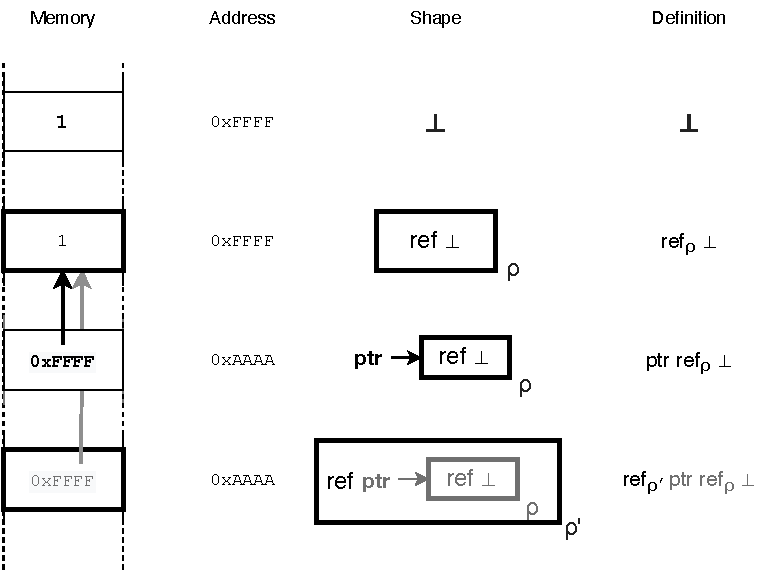
\includegraphics[width=0.7\textwidth]{background/figures/shapes}
    \caption{An illustration of \textit{shapes} and how they represent values in memory. Arrows represent pointers, and bold cells refer to the cell itself, not its contents.}
    \label{shapes-figure}
\end{figure}

\newpar A shape approximates the memory representation of an object, and this shape is fixed and kept across type casts. Shapes are annotated with regions showing a \texttt{"points-to"} relationship between references. Abal et. al. defines shapes in the following terms. 

\begin{equation*}
\begin{aligned}
    \text { l-value shapes } Z^L \quad &: \quad \text{ref}_{\rho} \:Z^R \quad | \quad \text{ref}_{\rho}\:(Z_1^L \times \cdots \times Z_n^L \stackrel{\varphi}{\rightarrow} Z_0^R)\\
    \text {r-value shapes } Z^R \quad &: \quad \perp \quad | \quad \text { ptr } Z^L \quad | \quad \zeta
\end{aligned}
\end{equation*} 

\noindent Shapes are also divided into l-value and r-value shapes in a similar fashion as the aforementioned type system, albeit without an integer type and with shape variables, $\zeta$. An r-value is the shape objects where the \textit{atomic} shape, $\perp$, indicates that an object has no relevant structure --- e.g. an integer. A pointer expression has the pointer shape, $\text{ ptr } Z^L$, where $Z^L$ is the shape of the target reference cell of the pointer. This means that a pointer represents the address of a reference cell, and therefore a pointer shape necessarily encloses a reference shape. If a pointer is being cast, its integer value will then have a pointer shape, $\text{ ptr } Z^L$. $\zeta$ represents arbitrary r-value shapes. These definitions and how they represent values in memory are illustrated in Figure \ref{shapes-figure}.

\newpar For functions, these function shapes are mapped to \textit{function shapes},

\begin{equation*}
    \operatorname{ref}_{\rho_{0}}\left(Z_{1}^{L} \times \cdots \times Z_{n}^{L} \stackrel{\varphi}{\rightarrow} Z_{0}^{R}\right).
\end{equation*} 

\newpar Function shapes represent an abstraction of the shapes given to a function as well as the shape of the result of the function. The parameters $Z_{1}^{L} \times \cdots \times Z_{n}^{L}$ correspond to the shapes of parameters the function is given and $Z_{0}^{R}$ is the shape of the result of the function. Since function parameters are stored in stack variables, these parameters are l-value shapes. The \textit{latent effect}, represented as $\stackrel{\varphi}{\rightarrow}$ above represents the effects that may happen when executing the function. These effects are described in the following section. Function shape schemes along with the correlation between types and shapes are described in more detail by Abal et. al. \cite{Abal2017EffectiveBF}. 

\newpar An environment $\Gamma$ maps variables $v$ to their corresponding reference shapes: $\Gamma(v) = ref_\rho Z$. $v$ is effect variables, described in the following. As already mentioned, function shapes are represent effects that may happen when executing a function, but this \textit{may} can be made more concrete using function inlining, in which case the actual effects of calling a function within another function can be inferred concretely. The use of inlining is detailed in Section \ref{implementation}. 

\subsection{Effects}
Effects represent how expressions affect regions. For example, an expression which reads a memory location will have the effect of reading that region. Likewise, expressions writing to memory locations will have the effect of writing to that region. An example of a set of effects is $\varphi = \{read_\rho , read_{\rho'} , write_{\rho'}\}$, where the region $\rho$ is being read and the region $\rho'$ is being both read and written.

\subsection{Shape-and-effect Inference}
Abal et. al. present inference rules $\vdash_{L} \subseteq \text { ENV } \times \text { L-VALUE } \times \text { SHAPE } \times \text { EFFECT }$ for \textit{shape-and-effect inference}, which allows determining what shape a given expressions has as well as determining what the effects of evaluation the expression are. This is expressed as the judgments: 

\begin{itemize}
    \item $\Gamma \vdash_{L} L: \text{ref}_{\rho} Z \& \varphi$, specifying that under $\Gamma$, the l-value expression $L$ has the shape $\text{ref}_\rho Z$, resulting in the effects $\varphi$
    \item $\Gamma \vdash_{E} E: Z \& \varphi$, specifying that under $\Gamma$, the r-value expression $E$ has the shape $Z$ resulting in the effects $\varphi$
\end{itemize}

\newpar Following the previous examples of effects, the $\text{FETCH}$ and $\text{ASSIGN}$ inference rules allow determining whether an expression will have the effect of reading or writing: 

\begin{equation*}
\begin{aligned}
    &[\text{FETCH}] \quad \frac{\Gamma \vdash_{L} L: \text{ref}_{\rho} Z \& \varphi}{\Gamma \vdash_{E} {!L}: Z \& \varphi \cup\left\{r e a d_{\rho}\right\}}\\
    &[\text{ASSIGN}] \quad \frac{\Gamma \vdash_{L} L: \mathrm{ref}_{\rho} Z \& \varphi_{1} \quad \Gamma \vdash_{E} E_{1}: Z \& \varphi_{2} \quad \Gamma \vdash_{E} E_{2}: Z' \& \varphi_{3}}{\Gamma \vdash_{E} L:=E_{1} ; E_{2}: Z^{\prime} \& \varphi_{1} \cup \varphi_{2} \cup\left\{w r i t e_{\rho}\right\} \cup \varphi_{3}}
\end{aligned}
\end{equation*}

Abal et. al. axiomize the behvaiour of certain operations, $f$, with a signature, $Z_{i}^{L} \stackrel{\varphi}{\rightarrow} Z_0$. The axiom specifies shapes of the input arguments expected by the function, $Z_{i}^{L}$, the shape of the output, $Z_0$, and the resulting effects, $\varphi$. The authors present an example of two axioms for locking and unlocking functions found within the Linux kernel: 

\begin{equation*}
\begin{aligned}
        \texttt{spin\_lock}: \quad & \text{ref}_{\rho_1} \text{ptr } \text{ref}_{\rho_2} \zeta \xrightarrow{{\texttt{lock}}_{\rho_2}}\perp \\
        \texttt{spin\_unlock}: \quad & \text{ref}_{\rho_1} \text{ptr } \text{ref}_{\rho_2} \zeta \xrightarrow{{\texttt{unlock}}_{\rho_2}}\perp
\end{aligned}
\end{equation*}

\newpar Axioms have been defined by Abal et. al. for multiple functions in the kernel, allowing inferring what the effects are of using these built-ins. These specify that \texttt{spin\_lock} and \texttt{spin\_unlock} receive pointers as arguments, $\rho_1$, pointing to an object, $\rho_2$. The effects above the arrows indicate that the functions \texttt{lock} and \texttt{unlock} the object in $\rho_2$, respectively.

\subsection{Effect-CFG Abstraction}
Abal et. al present the \textit{Effect-based Control-Flow Graph ($\varphi$-CFG)}. This is described as a CFG where nodes represent program locations and edges specify the control flow, annotated with variables with their memory shapes, and nodes with the effects inferred for their corresponding locations. 